% --------------------- VARIABLEN -------------------------

\newcommand{\COURSE}{Physik und Materialwissenschaften\\ Praktikum Physik \\}
\newcommand{\SEMESTER}{Elektro- und Informationstechnik II}
\newcommand{\STUDENT}{Maximilian Spahn\\ und\\Benjamin Langer}

\newcommand{\HEADDING}{Praktikum Physik}
\newcommand{\SUBHEADDING}{Versuch 4.3: Wärmestrahlung und Konvektion}

% ------------------- DEFINITIONEN -----------------------

\documentclass[a4paper]{scrartcl}

\usepackage[utf8]{inputenc}
\usepackage[ngerman]{babel}
\usepackage{amsmath}
\usepackage{amssymb}
\usepackage{color}
\usepackage{tikz}
\usepackage{float}
\usetikzlibrary{arrows,decorations.markings}
\usepackage{tabularx}
\usepackage{fancybox}
\usepackage{pgfplots}
\usepackage{geometry}
\usepackage{fancyhdr}
\usepackage[page]{totalcount}
\usepackage[colorlinks=true,linkcolor=black,urlcolor=blue,bookmarks,bookmarksopen=true]{hyperref}

%Größe der Ränder setzen
\geometry{a4paper,left=2cm, right=2cm, top=3cm, bottom=2cm, headheight=8cm}

%Kopf- und Fußzeile
\pagestyle {fancy}
\fancyhf{}
\fancyhead[L]{\STUDENT}
\fancyhead[C]{\COURSE}
\fancyhead[R]{\today}

\fancyfoot[L]{\SEMESTER}
\fancyfoot[C]{}
\fancyfoot[R]{Seite \thepage /\pageref{LastPage}}

%Formatierung der Überschrift, hier nichts ändern
\def\header#1#2{
  \begin{center}
    {\Large #1}\\
    {#2}
  \end{center}
}

\numberwithin{equation}{subsection}

\setlength\parindent{0pt}

% ----------------------- DOCUMENT ---------------------------

\begin{document}

\vspace{10pt}
\header{\HEADDING}{\SUBHEADDING}

\tableofcontents

\newpage

\section{Einleitung}

\newpage
\section{Theorie}

\newpage
\section{Häusliche Vorarbeit}
\subsection{Teil A: Wärmestrahlung}
\subsubsection{Beschreibung der Auslegung eines Kühlkörpers für optimale Wärmestrahlung}
Auf der Abbildung \ref{fig:kuehl} sieht man zwei verschiedene Möglichkeiten für die Rippenanordnung eines 
Kühlkörpers. Dabei ist die linke Variante besser als die rechte. Das liegt daran, dass durch die 
sternförmige Anordnung die Wärmestrahlung besser emittiert werden kann. Bei der Variante auf der rechten
Seite, wird die Wärmestrahlung zwar auch emittiert, aber durch die parallele Anordnung der Kühlrippen
wird ein Großteil der Strahlung wieder absorbiert. Dadurch kühlt die rechte Anordnung schlechter ab.

\begin{figure}[H]
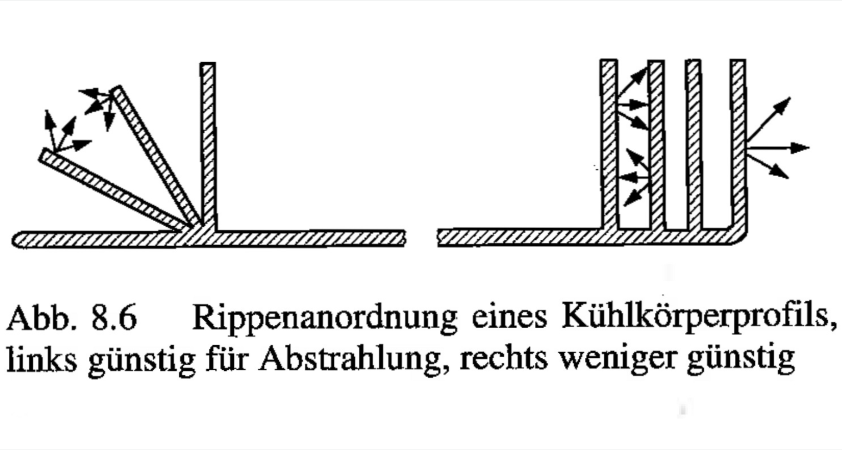
\includegraphics[width=12cm]{Abbildungen/Kuehlkoerper}
\centering
\caption{Beispiel von Leute für die Rippenanordnung von Kühlkörpern}
\centering
\label{fig:kuehl}
\end{figure}

\subsubsection{Berechnen der IR-Photonen}
Die Anzahl der IR-Photonen pro Sekunde werden mit der folgenden Formel berechnet:
\begin{align*}
N = \frac{I}{E} = \frac{I\cdot \lambda}{h\cdot c} = 20\;\frac{mW}{cm^2} \cdot 1\;\mu m \cdot 5,03\times 
10^{24} \approx 100,68\times 10^{15}
\end{align*}
\subsection{Teil B: Infrarotbildtechnik}
\subsection{Teil C: Konvektion}
\newpage
\section{Aufbau und Durchführung}

\newpage
\section{Auswertung Versuch}

\newpage
\section{Wertung/Fazit}

\newpage
\section{Anhang}

\newpage
\section{Literatur}

\label{LastPage}

\end{document}
%%% Local Variables:
%%% mode: latex
%%% TeX-master: t
%%% End:
